%!TEX root = ../../../report.tex
\section{Dimensional analysis} % (fold)
\label{sec:dimensional_analysis}
A problem came up when creating the robot. 
Some of the inertia moments obtained from SolidWorks, were in the order of magnitude of $10^{-8}$.
Such small number is not handled by the physics engine correctly causing the robot model to be unstable under normal conditions.

Three approaches were taken:
\begin{enumerate}
  \item \textbf{Change the physics engine}: As commented in the simulation comparison \ref{fig:simulation_comparison}, Gazebo supports multiple physics engines. Dart \cite{dart}, Simbody \cite{simbody}, Bullet \cite{bullet} and ODE \cite{ode}, where tested giving the same unstable behavior. 
  Thus, this method was discarded.
  \item \textbf{Fake the moments of inertia}: This would be to make 0 the really small moments of inertia and only leave the ones over a threshold.
  As the simulation is a qualitative analysis and no quantitative, an exact match of the moments of inertia is not needed. 
  \item \textbf{Dimensional analysis}: Based on \cite{dimensional_analysis}, the size of the robot can be increased in a proportion that make the figures big enough to be handled.
\end{enumerate}

Dimensional analysis can be applied to correlate the physical properties of the original robot with its scaled replica.
This is, is the original robot with mass $m$, volume $V$ and moment of inertia about an axis $I$, given a scale factor $s$, calculate the scaled replica $m'$, $V'$, $I'$ depending exclusively on $s$.

In the equation \ref{eq:general_inertia}, the generalized expression of the moment of inertia about an axis is shown.
\begin{equation}
\label{eq:general_inertia}
  I = \iiint_V \rho(u,v,w) |r^{2}| \,dx\,dy\,dz
\end{equation}

If the equation \ref{eq:general_inertia} is taken as the moment of inertia from the first link, the scaled one would be the shown in the equation \ref{eq:general_inertia_2}:
\begin{equation}
\label{eq:general_inertia_2}
  I' = \iiint_{V'} \rho(u,v,w)' |r^{'2}| \,dx'\,dy'\,dz'
\end{equation}

Supposing a scale factor of $s$ and as stated in the equations from \ref{eq:dx} to \ref{eq:dz}:

\begin{multicols}{3}
  \begin{equation}
  \label{eq:dx}
    \,dx=s \,dx'
  \end{equation}\break
  \begin{equation}
  \label{eq:dy}
    \,dy=s \,dy'
  \end{equation}\break
  \begin{equation}
  \label{eq:dz}
    \,dz=s \,dz'
  \end{equation}\break
\end{multicols}

Then can be deduced that $r$ increases proportionally with $s$ as shown in the figure \ref{fig:dimensional_analysis} and presented in the equation \ref{eq:dr}:
\begin{equation}
  \label{eq:dr}
  \,r=s \,r'
\end{equation}

\begin{figure}[ht!]
  \centering
  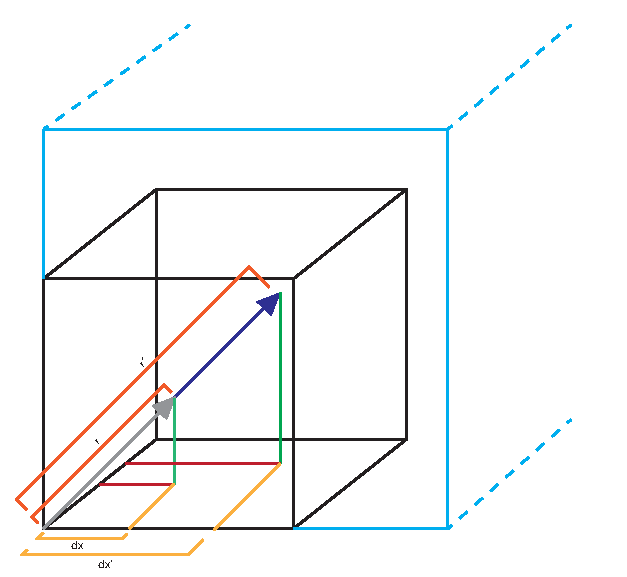
\includegraphics[width=0.5\linewidth]{figures/dimensional_analysis.pdf}
  \caption{Representation of a minimal volumentric cube.}
  \label{fig:dimensional_analysis}
\end{figure}

Assuming a constant density across all the scaled bodies, and particularizing for the moment of inertia of the center of gravity the moment of interia is given then by \ref{eq:general_inertia_3}:
\begin{equation}
  \label{eq:general_inertia_3}
  I'_{CG} = \iiint_{V'} \rho(u,v,w)' |r^{'2}| \,dx'\,dy'\,dz' = s^{3} r_{CG}^{'2} m
\end{equation}

A correlation can be obtained for the inertia then as shown in \ref{eq:inertia_scale}:

\begin{equation}
\label{eq:inertia_scale}
  I' = \frac{s^{3} r_{CG}^{'2} m}{r_{CG}^{2} m} I = s^{5} I
\end{equation}

And lately the mas can be correlated as in \ref{eq:mass_scale}:
\begin{equation}
\label{eq:mass_scale}
  m' = V' \frac{m}{V} = s^{3}m
\end{equation}

As explained in the \ref{sec:robot_definition}, by using the Xacro format, mathematical expressions can be used.
The definition of the robot includes a set of variables in which is included $scale$ that is used to calculate $mass\_scaled$ and $inertia\_scaled$ that will modify the values of all the links to make a coherence scalable robot definition.

% section dimensional_analysis (end)